
\begin{figure}[t]
    \centering
    \begin{subfigure}[b]{.24\linewidth}
        \centering
        \includegraphics[width=\linewidth]{figure/plot/reference/fig14-pmdk-kv-memory-pattern-256.tikz.pdf}
        \caption{[Ref] 256}
        \label{fig:14:ref:pmdk-kv-memory-pattern1}
    \end{subfigure}
    \hfill
    \begin{subfigure}[b]{.24\linewidth}
        \centering
        \includegraphics[width=\linewidth]{figure/plot/reference/fig14-pmdk-kv-memory-pattern-512.tikz.pdf}
        \caption{[Ref] 512}
        \label{fig:14:ref:pmdk-kv-memory-pattern2}
    \end{subfigure}
    \hfill
    \begin{subfigure}[b]{.24\linewidth}
        \centering
        \includegraphics[width=\linewidth]{figure/plot/reference/fig14-pmdk-kv-memory-pattern-768.tikz.pdf}
        \caption{[Ref] 768}
        \label{fig:14:ref:pmdk-kv-memory-pattern3}
    \end{subfigure}
    \hfill
    \begin{subfigure}[b]{.24\linewidth}
        \centering
        \includegraphics[width=\linewidth]{figure/plot/reference/fig14-pmdk-kv-memory-pattern-1024.tikz.pdf}
        \caption{[Ref] 1024}
        \label{fig:14:ref:pmdk-kv-memory-pattern4}
    \end{subfigure}
    \\
    \begin{subfigure}[b]{.24\linewidth}
        \centering
        \resizebox{\linewidth}{!}{\includegraphics{example-image-duck}}
        % \includegraphics[width=\linewidth]{figure/plot/reproduce/fig14-pmdk-kv-memory-pattern-256.tikz.pdf}
        \caption{[Rep] 1st month}
        \label{fig:14:rep:pmdk-kv-memory-pattern1}
    \end{subfigure}
    \hfill
    \begin{subfigure}[b]{.24\linewidth}
        \centering
        \resizebox{\linewidth}{!}{\includegraphics{example-image-duck}}
        % \includegraphics[width=\linewidth]{figure/plot/reproduce/fig14-pmdk-kv-memory-pattern-512.tikz.pdf}
        \caption{[Rep] 512}
        \label{fig:14:rep:pmdk-kv-memory-pattern2}
    \end{subfigure}
    \hfill
    \begin{subfigure}[b]{.24\linewidth}
        \centering
        \resizebox{\linewidth}{!}{\includegraphics{example-image-duck}}
        % \includegraphics[width=\linewidth]{figure/plot/reproduce/fig14-pmdk-kv-memory-pattern-768.tikz.pdf}
        \caption{[Rep] 3rd month}
        \label{fig:14:rep:pmdk-kv-memory-pattern3}
    \end{subfigure}
    \hfill
    \begin{subfigure}[b]{.24\linewidth}
        \centering
        \resizebox{\linewidth}{!}{\includegraphics{example-image-duck}}
        % \includegraphics[width=\linewidth]{figure/plot/reproduce/fig14-pmdk-kv-memory-pattern-1024.tikz.pdf}
        \caption{[Rep] 1024}
        \label{fig:14:rep:pmdk-kv-memory-pattern4}
    \end{subfigure}
    \caption{PMDK key-value store's memory access pattern when updating different key-value pairs.}
    \label{fig:14:pmdk-kv-memory-pattern-feature}

\end{figure}
